\section{Push Server: the APE Server} % (fold)
\label{sec:ape}

Because of technical limitations of traditional browsers, it is not trivial to develop real time applications with \idx{JavaScript}.
More precisely, since it cannot directly push data from the server to the browser, the only native solution is to poll in regular time intervals --- an inefficient approach.

The apprehended solution in the old system was to embed a \idx{Java applet} solely to communicate with the server.
The \idx{Java} \ida{API} for applets includes support for sockets, so it is possible to pass data in real time.
However, the big drawback is that it needs the \idx{Java} plugin to be installed in browsers, and there is no plugin for mobile browsers --- neither in \idx{iOS} nor in \idx{Android}.

It was decided that mobile browsers must be supported by the second iteration of this project, so a new solution native to those browsers should be considered, getting rid of this \idx{Java applet}.

\subsection{Comet} % (fold)
\label{sub:comet}

Shortly after \ida{AJAX} was popularized, another technique ---called in contrast \idx{Comet}--- was developed to solve the particular use case of pushing data from the server to the client.
Since then, several alternatives for creating real-time applications have been developed:

\begin{figure}[htbp]
  \centering
    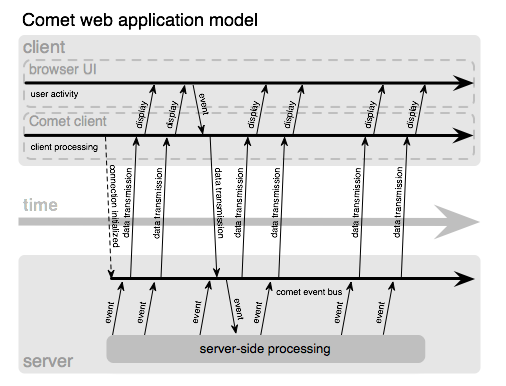
\includegraphics[width=\textwidth]{comet-flow}
  \caption[Comet flow]{Typical flow in a Comet application (compare with Figure~\vref{fig:ajax-flow})\newline© Alex Russell / \url{infrequently.org})}
  \label{fig:comet-flow}
\end{figure}

\begin{description}
  \item[\idx{WebSocket} \ida{API}] An \ida{HTML}5 extension\footnote{\url{http://dev.w3.org/html5/websockets/}} easy to use that just offers a socket to any server.
  This would be the perfect choice (and it should be chosen in the future), but at the moment it severely lacks support among the supported browsers, so it cannot be considered.
  \item[\idx{Socket.IO}] Since real sockets in browsers are out of the equation, an application with both browser and server components is the only way to go.
  One of the options with a brighter future relies on \idx{NodeJS}\footnote{\url{http://nodejs.org/}}, an effort to bring \idx{JavaScript} to the server.
  
  \idx{Socket.IO}\footnote{\url{http://socket.io/}} is a simple software that simulates real sockets in the browsers and uses \idx{NodeJS} for its server component.
  It holds quite interesting ideas, but it was discarded because then it was in a pretty immature state.
  \item[\idx{CometD}] This is a similar approach by the \idx{Dojo} Foundation\footnote{\url{http://cometd.org/}} (so it works well with the dojo framework), creating a new protocol called Bayeux\footnote{\url{http://svn.cometd.com/trunk/bayeux/bayeux.html}}.
  In a quick glance it was rejected because it seems too complex for this task, and it could end in adding an additional framework in the mix.
  \item[\ida{APE} server] And finally we get to the winner of our contest.
  The \ida{APE} project\footnote{\url{http://www.ape-project.org/}} is a solid full solution with two components (server/browser), and it is focused on supporting real time data streaming.
  Just visiting its website explains why it seems like a better solution, because of the extensive documentation and well-explained examples --- from simple to advanced ones.
  
  One of the reasons why it was chosen it that it offers many layers of tinkering.
  If we only want a socket to a existing server, it has a proxy socket built so it is not needed to write any additional server code.
  But if we need to develop an advanced application, custom modules for the server can be written in \idx{JavaScript}.
  
  The other big reason is that it is written with \idx{MooTools}, so bringing \ida{APE} to the table bears little overhead for the client code.
  In the server, a hypothetical custom module could benefit from having the same framework as in the browser.
\end{description}

After considering all options, the \ida{APE} project looked the most promising one.
Eventually, just the proxy socket was needed, so it was merely a drop-in replacement for the \idx{Java applet}.
In any case, as its server deployment (see \S\vref{sec:deployment}) consists on almost exclusively installing the \idx{Debian} \ida{APE} package, it results in an elegant and painless solution.

% subsection comet (end)

\subsection{How the APE Server Works} % (fold)
\label{sub:how_the_ape_server_works}

As we said, the system needs two components: one to be installed in the server and a script to be included in our web application.
The first component is a typical web server that listens upon a port, with the special peculiarity that only understands the \ida{APE} protocol.

\begin{wrapfigure}{r}{0.5\textwidth}
  \centering
    
\includegraphics[width=0.48\textwidth]{ape-comic}
  \caption{Real official APE documentation}
  \label{fig:ape-comic}
\end{wrapfigure}

In that server, modules can be written in \idx{JavaScript} (or even \idx{C}), with a convenient \ida{API} to access common web resources like sockets, pipes or \idx{MySQL} connections.
There are some modules and plugins implemented by default, like one that acts as a proxy for \ida{TCP} sockets, or other that redirects data from a server application to the client.
With those two simple modules a lot of applications can be written without needing a custom module.

The server maintains a list of named channels; each channel holds one or more users that can write and read from that channel.
Again, every user can have more than one connection, for example a user that has two tabs open in the same browser, or that have two sessions in two different devices at the same time.
For this, the server \ida{DNS} must be configured to answer to multiple dynamic subdomains  (\verb|1.ape.domain.com|, \verb|2.ape.domain.com|, \verb|42.ape.domain.com|, etc).

In the browser, a set of scripts must be added to our web application so that they can talk with the backend: the \ida{APE} \ida{JSF}.
The configuration is very basic: it only needs the \ida{URL} for the rest of the scripts and the base domain of the \ida{APE} server.

\begin{lstlisting}[language=JavaScript,label=apesocket,caption=TCPSocket usage in APE JSF]
var client = new APE.Client();
var socket;

client.load();
client.addEvent('load', function() {
  this.core.start();
});

client.addEvent('ready', function() {
  socket = new this.core.TCPSocket();
  socket.open(host, port);
  socket.onopen = function() {
    socket.send('hello world');
  };
  socket.onread = function(msg) {
    console.log('New message: ' + msg);
  };
  socket.onclose = function() {
    socket = null;
    console.log('Connection with the server closed.');
  };
}

window.addEvent('unload', function() {
  socket.close();
}
\end{lstlisting}

Then the \ida{APE} client can be created, the connection opens and the two parties start exchanging messages.
Messages are formatted as \ida{JSON} arrays that contains two groups of objects: \emph{commands} and \emph{raws}.
The former ones come from browsers to the server while the latter ones go the other way around.

Commands should be taken as actions that the clients want to accomplish, like opening the connection or sending some data.
Commands are composed by a name, a challenging number (increased each time, to numerate the messages) and optional parameters.
Depending on the name, the message is processed by the very \ida{APE} server or served to a custom module that will answer to that action.

Raws can be expressed as data sent by the server, indeed it is composed by a name, a timestamp and the data as a \ida{JSON} object.
Again, the name reveals the purpose of the transmission and the data format.
It is not uncommon for a message (that is, a \ida{JSON} array) to contain more than one raw.

To send a command, the client creates a \idc{GET} or \idc{POST} request to a increasingly numerated subdomain, encoding the \ida{JSON} array as the only parameter.
When there is data to send, the server answers and the raw(s) can be found in the body response.

% subsection how_the_ape_server_works (end)

\subsection{Transport Methods} % (fold)
\label{sub:transport_methods}

Though it is not completely essential to know how exactly the \ida{APE} server works in the backend, it should be understood how it earns its push capabilities.
There are four transport methods implemented that the developer can choose from, but each of them has its strengths and weaknesses.

\begin{description}
  \item[\idx{Long-polling}] This is the default transport method (so it will be selected unless noted otherwise), and it works in pretty much every \idx{JavaScript}-enabled browser.
  It is based on \ida{AJAX} but with a twist: the client request a resource but the server keeps the \ida{HTTP} connection open until it has something to say.
  
  When there is data to send (or after a certain timeout), the server sends the response.
  Then, the client immediately re-request the same resource, so the server has always a connection open to the browser.
  Of course, the main drawback of this approach is that it is more like a hack, so it could be done more efficiently.
  \item[\ida{JSONP}] Similar to the previous one but over \ida{JSONP} instead of \ida{AJAX}, so it offers cross-domain possibilities.
  \item[\idx{XHRStreaming}] Also very similar to the first one, with the exception that the server do not close the connection when it has information to send.
  Therefore it only needs one connection, so it is more efficient.
  Sadly, this only works with recent browsers.
  \item[\idx{WebSocket}] As said before, this only works in a few new browsers, so it does not make sense to support it just yet if most times it is going to fallback to the default transport method.
\end{description}
% subsection transport_methods (end)
% section ape (end)